\pagestyle{fancy}
\lhead{}
\renewcommand{\chaptermark}[1]{\markboth{\thechapter.\ #1}{}}

\chapter{Nonlinear effects}
\label{ch:nonlinearEffects}

There is a great scientific and technological interest in Silicon for developing photonic devices based on nonlinear processes. Table \ref{tab:nonlinearDevices} contains a selection of the most important works on the subject for the last six years.
These works can be classified according to the main nonlinear effect observed in Silicon:

\begin{itemize}
\item \textbf{Thermal effects} are the slowest (ms).
Light can heat silicon, and an increase in temperature increases its refractive index. Its coefficient is equal to $1.8 \times 10^{-4}/^\circ$C~\cite{Pruessner2007,Kiyat2006}. This effect can be beneficial in some applications where fine tuning is necessary, which can be achieved by applying temperature variations. On the other hand, this effect can be problematic when a stable performance with temperature is desired. In those cases, one can introduce a cladding material with a negative thermo-refractive coefficient in order to make the device athermal~\cite{Teng2009,Zhou2009a,Han2007}.

\item \textbf{Free carrier effects} \cite{Almeida2004,Boyraz2004,Preble2005,Liang:05,Foster2007,Waldow2008} appear at relatively high powers ($>$100~mW for the geometries presented in the thesis) and are generated through two-photon absorption (TPA). They produce changes both in refractive index (free-carrier-dispersion, FCD) ($\Delta n < 0$) and absorption (free-carrier absorption, FCA) that can be used for switching one beam using another co-propagating beam. The problem is that the carriers take nano-seconds to recombine, limiting the switching to around 1~GHz speed.


\item \textbf{Kerr effect} \cite{Hochberg2006,Martinez2010} is produced by the third order nonlinear coefficient $\chi^{(3)}$, and has the advantage of having instantaneous response time, which introduces no speed limitations.
The problem is that the power levels needed also create carriers through TPA, and these carriers hinder the Kerr effect.
One strategy to increase the Kerr response is to include materials with a high $\chi^{(3)}$ in the waveguide section. Another possibility is to use amorphous silicon, which has a lower TPA coefficient and very fast carrier recombination time~\cite{Matres2013}.

\item \textbf{Pockels effect} is produced by the second order nonlinear coefficient, $\chi^{(2)}$. The problem is that it appears only in materials with no inversion center, such as $\mathrm{LiNbO}_3$, and in silicon, is zero. However, depositing a $\mathrm{Si_3N_4}$ layer, one can induce stress and break the symmetry of Silicon~\cite{Jacobsen2006,Cazzanelli2012,Chmielak2011}.
\end{itemize}

\begin{table}
\centering
\begin{tabulary}{1.00\textwidth}{|L|L|L|L|L|}\hline 
\textbf{Ref.} & \textbf{Group} & \textbf{Structure} & \textbf{Effect} & \textbf{Details}\\ \hline
\cite{Almeida2004b} & Cornell & Ring & carriers (FC) generated through TPA & 450~ps response\\ \hline
\cite{Boyraz2004} & UCLA & Mach-Zehnder & Kerr + FC & 7~ns response due to carriers\\ \hline
\cite{Preble2005}& Cornell & Ring & FC generated through TPA & 7~ns response due to carriers\\ \hline
\cite{Liang:05}& IMEC - Ghent  & Waveguide & XAM & 13~ps response, 2~W peak power\\ \hline
\cite{Hochberg2006}& Caltech  & Si+ polymer & kerr & 1~ps response, 50~mW peak power but only 0.3dB modulation\\ \hline
\cite{Jacobsen2006} & Tech. Univ. of Denmark  & Si with strain & $\chi^{(2)}$ induced through strain &  measurement $\chi^{(2)} =15~$pm/V \\ \hline
\cite{Foster2007} & Cornell  & Ring & FC generated by TPA & 1~ns response, 30~mW peak power 	\\ \hline
\cite{Waldow2008} & Aachen Univ.  & Ring & fast carriers thanks to O implantation & 25~ps response with non-guided pump (800~nm) 	\\ \hline
\cite{Lee2009} & Cornell  & Waveguide & FWM & 40~Gbps conversion, 15~dB efficiency 	\\ \hline
\cite{Koos2009} & Kalsruhe Univ., IMEC  & Si slot with polymer & FWM & 3~ps response	\\ \hline
\cite{Martinez2010}& Univ. Politec. Valencia & Ring (slot waveguide with Si-nanocrystals)  & kerr & 10~ps response 	\\ \hline
\end{tabulary}
\caption{Recent impact contributions in the area of nonlinear silicon photonics.}
\label{tab:nonlinearDevices}
\end{table}



\section{Kerr effect}
% Kerr effect is produced by the third order nonlinear $\chi^3$ coefficient and is the most desired due to its high speed ($10^{-15}~\mathrm{s}$).
% Kerr effect is produced by the third order nonlinear $\chi^3$ coefficient, that has a quadratic dependence on the electric field ($\Delta n = \lambda K E^2$ ), where $\lambda$ is the wavelength of the light, K is the Kerr constant, and E is the strength of the electric field

Kerr effect produces a refractive index change ($\Delta n = n_2 I$) that depends on the optical intensity (I) and nonlinear refractive index ($n_2$). For silica, $n_2$ is typically in the order of $2.7\times10^{-16} \mathrm{cm^2/W}$ , whereas in Silicon, it is significantly higher ($4.5\times10^{-14} \mathrm{cm^2/W}$) \cite{Dinu2003a}.
Moreover, the strong confinement of the mode in small waveguides, enhances nonlinear effects, so it is more convenient to use the nonlinear coefficient ($\gamma$) definition:

\begin{equation}
 Re(\gamma) = \frac{n_2\omega}{cA_{eff}}
\label{eq:gamma}
\end{equation}

where the effective area ($A_{eff}$) is defined as in paper~\cite{Rukhlenko2012}:

\begin{equation} 
  A_{eff}= \frac{(\iint |E(x,y)|^2 dxdy)^2}{\iint |E(x,y)|^4 dxdy}
\label{eq:aeff}
\end{equation}


Kerr effect is the most desired due to its high speed ($10^{-15}~\mathrm{s}$).
However it is a very weak effect that requires power densities higher than Free carrier generation, so it is masked by the effects of these carriers.
It can be maximized with structures that confine the power in a small area, such as slot waveguides~\cite{Martinez2010}, or combining silicon with other materials with a higher $\chi^3$ coefficient, such as silicon nano-crystals~\cite{Spano2009} or some polymers~\cite{Koos2009}.
Since the Kerr constant of silicon is positive it produces an increase in refractive index ($\Delta n > 0$) and is responsible for the nonlinear optical effects of Four Wave Mixing (FWM), Self-phase modulation (SPM) and Cross-phase modulation (XPM).

\begin{itemize}
\item \textbf{Four Wave Mixing (FWM)} is a nonlinear effect in which using two wavelengths, two other are generated on both sides of the spectrum.
It is a phase-sensitive process, so the interaction depends on the relative phases between both signals and can accumulate over long distances when they satisfy a phase-matching condition, which depends on the wavelength separation and the even dispersion coefficients ($\beta_2$, $\beta_4$ , etc.).
In other cases, where there is a strong phase mismatch, four-wave mixing is not efficiently generated.
Moreover, free carrier generation also limits its efficiency.
There are several applications of FWM, such as generation of new frequencies~\cite{Bayvel1989}, wavelength conversion~\cite{Inoue1992,Lee2009} and parametric amplification \cite{Carman1966,Stolen1982,Foster2006}.

\begin{figure}[htb]
    \centering
    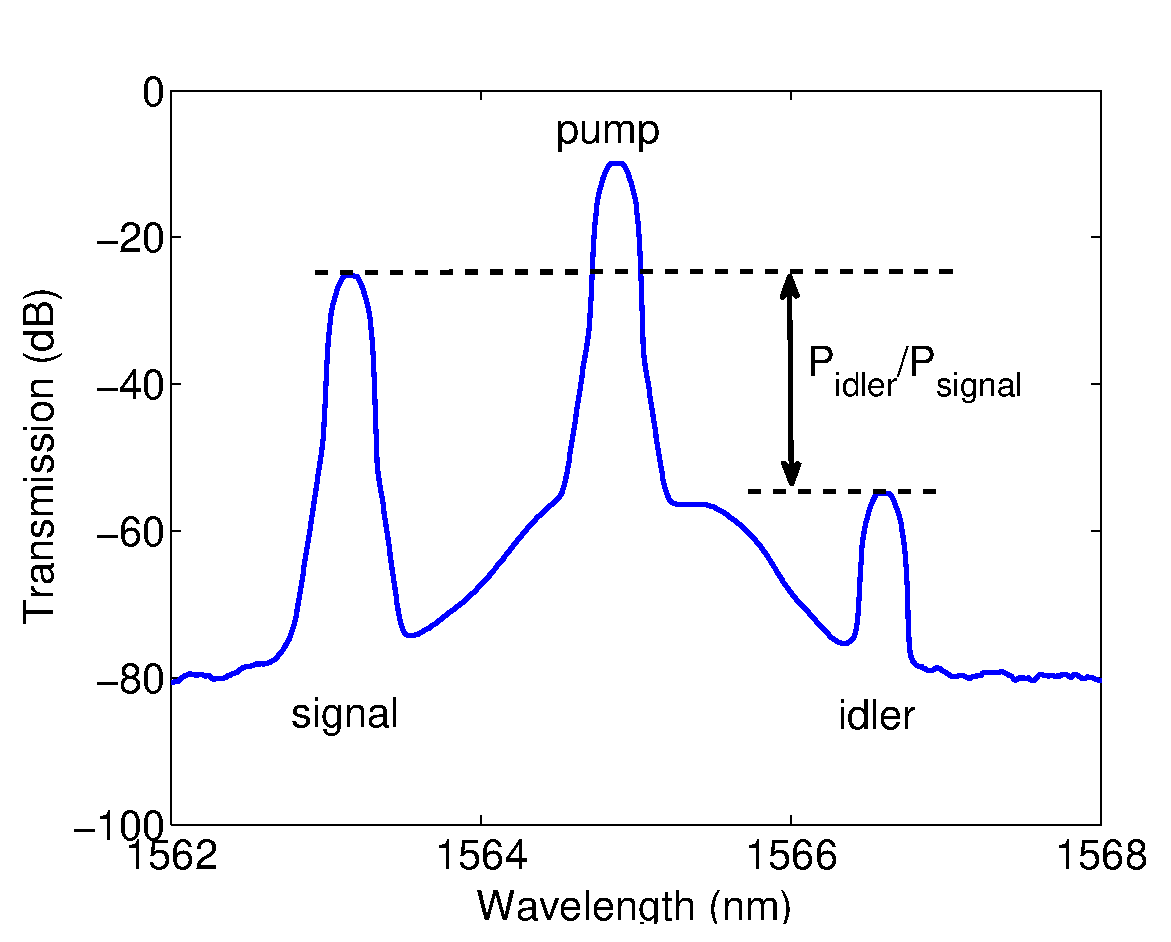
\includegraphics[width=\fWidth\textwidth]{Power_dBm_fwm_convEffMax_29p5dB}
    \caption{Generation of new frequency components via four-wave mixing.}
    \label{fig:fwmMaxEfficiency}
\end{figure}

\item \textbf{Self-phase modulation (SPM)} takes place when a short pulse of light travels in a material and induces a refractive index change during its propagation due to kerr effect. This induced chirp broadens the spectrum of the pulse as it travels. One application of SPM is the generation of super-continuum using ultrashort high peak power pulses and a nonlinear media~\cite{Boyraz2004}.

\item \textbf{Cross-phase modulation (XPM)} is a more interesting effect in terms of switching. We can use one signal to induce a refractive index change in a waveguide where another signal is traveling. Through those changes we can control one beam using another beam, changing, for example, the phase relationship between the arms of a Mach Zehnder Interferometer or the phase of a beam traveling inside a ring resonator.

\end{itemize}



\section{Two photon absorption (TPA)}
For all-optical switching, the desirable Kerr effect is limited by Two photon absorption (TPA), due to the absorption of two photons whose energy is transfered to excite an electro-hole pair.
In a waveguide, we can consider it as the imaginary part of the gamma coefficient:

\begin{equation}
 \frac{dP}{dz} = -\alpha P(z) - 2|Im(\gamma)| P(z)^2 
\label{eq:differentialTPAImGamma}
\end{equation}

where $\alpha$ and $Im(\gamma)$ are the linear and nonlinear loss and P is the power of the signal through the waveguide.

The Figure of Merit (FOM) measures the ratio between the nonlinear coefficient $Re\{\gamma\}$ and nonlinear absorption $Im\{\gamma\}$, and must be larger than two for efficient all-optical switching~\cite{Vallaitis2009,Delong1989,Mizrahi}.
We measure $Re\{\gamma\}$ through four wave mixing (appendix~\ref{ch:fwm}) and $Im\{\gamma\}$ from the nonlinear loss measurements (\ref{ch:imGamma}).
\textit{Vallaitis et al} present a way to determine a Figure of Merit which is valid without having to estimate any peak power, effective area, waveguide effective length or absorption coefficient. It only uses the nonlinear phase shift ($\Delta\phi_{NL}$) and the amplitude transmission ($T_A$) from the nonlinear time resolved measurements (\ref{ch:timeRes}):


\begin{equation} 
FOM_{TPA}=\frac{-1}{4\pi} \frac{Re\{\gamma\}}{Im\{\gamma\}} = -\frac{\Delta\phi_{NL}}{4\pi lnT_A}
\label{eq:fom}
\end{equation}

% We have mentioned several nonlinear behaviors with different characteristics. Some are desirable ($Re\{\gamma\}$) but others are not ($Im\{\gamma\}$). We must then define a way to determine the quality of the nonlinear behavior in each sample given by the Figure of Merit (FOM). Equation 1, developed in paper [2], presents a way to determine a Figure of Merit which is valid without having to estimate any peak power, effective area, waveguide effective length and absorption coefficient.

\section{Free carrier effects}
Free carriers are generated in the silicon by Two photon absorption (TPA).
We can basically differentiate two different carrier effects, all of which originate from the same TPA phenomena:

\begin{itemize}
\item \textbf{Free carrier dispersion (FCD)} produced by the refractive index change of the carriers. 

\item \textbf{Free carrier absorption (FCA)} because the excess of carriers absorb light. 
However, using a reverse polarized junction~\cite{Turner-Foster2010} or implanting dopants~\cite{Liu2006}, one can reduce the carrier lifetime and the effect of FCA.
\end{itemize}

At 1550~nm we can use the empirical formulas of free carriers, where $n_f$ is the free-carrier index (FCI) and $\alpha_f$, expressed in $cm^{-1}$, governs the free carrier absorption (FCA)~\cite{Lin2007,Soref1987}:

% \begin{equation} 
% \chi = 2n_0[n+jc\alpha/(2\omega)]
% \label{eq:chi}
% \end{equation}

\begin{equation} 
n_f = -(8.8\times 10^{-4}N_e+8.5N_h^{0.8})\times 10^{-18}
\label{eq:fcd}
\end{equation}

\begin{equation} 
\alpha_f = 1.45\times 10^{-17} N
\label{eq:fca}
\end{equation}

Carrier densities of holes ($N_h$) and electrons ($N_e$) generated through TPA are equal ($N_h=N_e=N$) and have $cm^{-3}$ units.
The negative sign in $n_f$ means a refractive index decrease due to free-carrier dispersion ($\Delta n<0$).


%Where carrier densities of holes ($N_h$) and electrons ($N_e$) are generated with equal densities through TPA ($N_h=N_e=N$) and have units of $cm^{-3}$.
%The negative sign in $n_f$ means a refractive index decrease due to free-carrier dispersion ($\Delta n<0$).

% In silicon at 1550~nm, a carrier density (N) produces free-carrier dispersion ($n_f = -5.3\times 10^{-21} N$) and absorption ($\alpha_f = 1.45\times 10^{-17} N$
%Where the carrier densities of holes ($N_h$) and electrons ($N_e$)  and are both generated with equal densities through TPA ($N_h=N_e=N$).
% \begin{equation} 
% FCI = -5.3\times 10^{-21} N
% \label{eq:fcd}
% \end{equation}
% 

% 
% Where N is the carrier density.

For all-optical switching, carriers can be the problem or the solution, according to the strategy employed.
If one managed to reduce the recombination time of carriers from 1~ns to tens of ps, the effect would be ideal for switching.
In samples fabricated through ePIXfab platform, this time was around 10~ns, while we also reported Silicon strip waveguides with recombination times in the order of 100~ps fabricated in our facilities~\cite{Oton,optoel}.
The recombination time of free carriers depends on several factors, such as dopant concentration or waveguide geometry.
Implanting dopants, such as Helium~\cite{Liu2006}, or using rib waveguides~\cite{Dimitropoulos2005} can increase the carrier diffusion and reduce carrier lifetime.
Another possibility is sweeping carriers with a p-i-n union inversely polarized, which considerably complicates the fabrication and increases the power consumption~\cite{Turner-Foster2010}.
Finally, slot \cite{Matres:12} and amorphous silicon waveguides~\cite{Matres2013} have demonstrated to reduce carrier associated effects.


\pagestyle{plain}
\bibliographystyle{unsrt}
\bibliography{library}

